\chapter{Obsah CD}
Na priloženom CD sa nachádzajú nasledovné súbory a~adresáre:
\begin{itemize}
\item \textbf{doc -} zdrojové súbory tohoto textu v~\LaTeX-ovom formáte 
spolu s~elektronickou verziou vo formáte PDF
\item \textbf{src -} zdrojové súbory plánovača testov spolu s~hlavičkami 
testov používaných v~praxi
\item \textbf{README.txt -} textový súbor obsahujúci príklady spustenia
\end{itemize}

\chapter{Ukážka jednoduchého plánu testov}
\label{priloha:jednoduchy_plan_testov}
Na nasledujúcej strane je zobrazený plán testov z~produktu MCO,
ktorý pozostáva z~desiatich clusterov. Z~obrázku vyplýva, že pre potreby
týchto clusterov je potrebné spustiť celkovo 19 prerekvizít a~19 
odrekvizít. Pre otestovanie produktu týmito desiatimi clustermi je 
potrebné vykonať ďalších 38 testov, ktoré slúžia na zmenu konfigurácie
systému a~na obnovu týchto zmien. 

Uvedený plán obsahuje celkovo 48 testov a~je relatívne jednoduchý.
V~regresných testoch sa aktuálne používa plán testov, ktorý v~prípade 
produktu MCO pozostáva z~viac ako 3100 testov.
Plán testov každodenne používaný v~regresnom testovní produktu SMSCv5 
pozostáva z~približne 3000 testov.

Príkaz pre naplánovanie a~spustenie regresnej sady každodenne 
používanej v~produkte MCO je zobrazený na obrázku 
\ref{obrazok:priklad_spustania_testov}.


\begin{figure}[h]
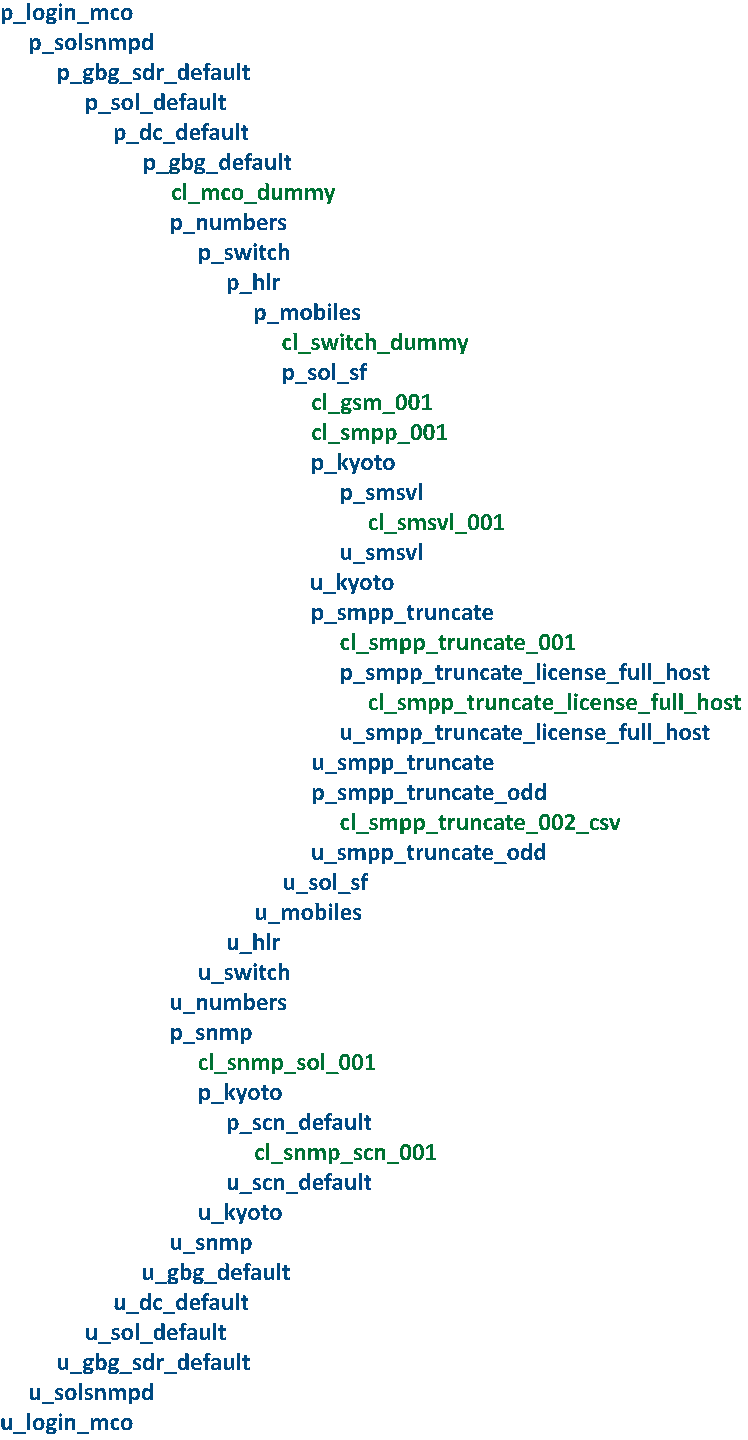
\includegraphics[scale=0.90]{ukazka_jednoducheho_planu}
\caption{Ukážka jednoduchého plánu testov}
\end{figure}

%\chapter{Konfigrační soubor}
%\chapter{RelaxNG Schéma konfiguračního soboru}
%\chapter{Plakat}

